%%%%%%%%%%%%%%%%%%%%%%%%%%%%%%%%%%%%%%%%%
% University Assignment Title Page 
% LaTeX Template
% Version 1.0 (27/12/12)
%
% This template has been downloaded from:
% http://www.LaTeXTemplates.com
%
% Original author:
% WikiBooks (http://en.wikibooks.org/wiki/LaTeX/Title_Creation)
%
% License:
% CC BY-NC-SA 3.0 (http://creativecommons.org/licenses/by-nc-sa/3.0/)
% 
% Instructions for using this template:
% This title page is capable of being compiled as is. This is not useful for 
% including it in another document. To do this, you have two options: 
%
% 1) Copy/paste everything between \begin{document} and \end{document} 
% starting at \begin{titlepage} and paste this into another LaTeX file where you 
% want your title page.
% OR
% 2) Remove everything outside the \begin{titlepage} and \end{titlepage} and 
% move this file to the same directory as the LaTeX file you wish to add it to. 
% Then add \input{./title_page_1.tex} to your LaTeX file where you want your
% title page.
%
%%%%%%%%%%%%%%%%%%%%%%%%%%%%%%%%%%%%%%%%%
%\title{Title page with logo}
%----------------------------------------------------------------------------------------
%	PACKAGES AND OTHER DOCUMENT CONFIGURATIONS
%----------------------------------------------------------------------------------------
\documentclass[UTF-8,12pt]{article}
\usepackage[UTF8]{ctex}
\usepackage[english]{babel}
\usepackage[utf8x]{inputenc}
\usepackage{amsmath}
\usepackage{graphicx}
\usepackage[colorinlistoftodos]{todonotes}

\begin{document}

\begin{titlepage}

\newcommand{\HRule}{\rule{\linewidth}{0.5mm}} % Defines a new command for the horizontal lines, change thickness here

\center % Center everything on the page
 
%----------------------------------------------------------------------------------------
%	HEADING SECTIONS
%----------------------------------------------------------------------------------------

\textsc{\LARGE \bfseries 中山大学 }\\[0.3cm] % Name of your university/college
\textsc{\Large 数据科学与计算机学院}\\[0.5cm] % Major heading such as course name
\textsc{\Large 软件工程}\\[0.3cm] % Major heading such as course name
\textsc{\Large 人工智能}\\[0.5cm]
 % Minor heading such as course title

%----------------------------------------------------------------------------------------
%	TITLE SECTION
%----------------------------------------------------------------------------------------

\HRule \\[0.4cm]
{ \huge \bfseries 遗传算法实验报告}\\[0.03cm] % Title of your document
\HRule \\[1.5cm]

 
%----------------------------------------------------------------------------------------
%	AUTHOR SECTION
%----------------------------------------------------------------------------------------

\begin{minipage}{0.4\textwidth}
\begin{flushleft} \large
\emph{Submitted By:}\\
徐伟元 16340261\\
熊永琦 16340258\\
李天译 16340122
\end{flushleft}
\end{minipage}
~
\begin{minipage}{0.5\textwidth}
\begin{flushright} \large
\emph{Submitted To:} \\
王甲海\\ 教授\\ 大数据与计算智能研究所 % Supervisor's Name
\end{flushright}
\end{minipage}\\[1cm]

% If you don't want a supervisor, uncomment the two lines below and remove the section above
%\Large \emph{Author:}\\
%John \textsc{Smith}\\[3cm] % Your name

%----------------------------------------------------------------------------------------
%	DATE SECTION
%----------------------------------------------------------------------------------------

{\large 2019-1-11}\\[1cm] % Date, change the \today to a set date if you want to be precise

%----------------------------------------------------------------------------------------
%	LOGO SECTION
%----------------------------------------------------------------------------------------


\includegraphics[width=2in]{logo.png}\\[0.5cm] % Include a department/university logo - this will require the graphicx package
 
%----------------------------------------------------------------------------------------

\vfill % Fill the rest of the page with whitespace

\end{titlepage}


\begin{abstract}
本实验利用遗传算法实现 TSP 问题求近似解,并提供图形化界面以及和使用相同局部搜索操作的模拟退火算法进行对比。

\end{abstract}


\section{实验题目}

用遗传算法求解 TSP 问题(问题规模等和模拟退火求解 TSP 实验同),要求:

\begin{enumerate}
    \item 设计较好的交叉操作,并且引入多种局部搜索操作(可替换通常遗传算法的变异操作)
    \item 和之前的模拟退火算法(采用相同的局部搜索操作)进行比较
    \item 得出设计高效遗传算法的一些经验,并比较单点搜索和多点搜索的优缺点
\end{enumerate}

\section{遗传算法}
\subsection{遗传算法原理}
遗传算法是受遗传学中自然选择和遗传机制启发发展起来的一种搜索算法,在每一代中,使用上一代最适应环境的位或片段,形成新的人工生物集。遗传算法虽然是随机化方法,但是它利用历史信息推测新的搜索点,使得搜索过程更为有效。

遗传算法在每一次迭代中保留一组候选解,并按照某种指标进行选择,再利用遗传操作对这些选出的候选解进行运算,产生新的一组解,重复这个过程直到满足指定的收敛要求为止。

\subsection{邻域操作}
为了更好地与模拟退火算法进行比较,我们使用模拟退火算法中采用的相同邻域操作替换通常遗传算法中的简单变异操作。即:

\begin{enumerate}
    \item 随机选择两个节点,交换其在队列中的位置
    \item 随机选择三个节点,轮换其在队列中的位置
    \item 随机选择两个节点,使得其间的节点次序反向
    \item 完全随机生成一个路径序列
\end{enumerate}

\subsection{选择}
有多种选择的方式可以选择,在本次试验中我们选择了 k = 2 的锦标赛方法(有放回),即在种群中每次随机选择 2 个不同个体,选择其中适应值较大的个体加入交配池,重复这一过程直到交配池中个体数与设定的种群大小相等。

\subsection{交叉}
我们采用两点交叉的算子。以一定交叉率进行,随机在交配池中选择两个父代,并随机选择两个交叉点,交换两个父代两点之间的基因片段,然后对结果再进行一次搜索替换掉基因由于交叉操作产生重复的城市,将产生的两个子代放回种群。交叉后的亲本依然留在种群中,便于后面的选择操作可以有更多可选解空间。

\subsection{变异}

以一定变异率在种群全体中选择一个个体进行变异,按照实验要求,使用前面提到的邻域操作替换通常使用的简单变异操作。在种群迭代过程中在几种邻域操作的解空间中各取出一个解,并选择其中最好的解替换原来的个体值。

\subsection{参数选择}
为了使种群具有更强的可控性,同时减少每一代的种群操作时间,但还要保证每代生成足够多的解模式,选择合理的种群大小是有必要的。

对于交叉率的选取,过高的交叉率可能会使较好的性状迅速丢失,而过低则不利于搜索的进行。

遗传算法也需要好的变异操作来维持种群多样性,变异率过大可能导致算法趋于随机搜索,而过小则可能使一些表现较好的基因丢失。由于本实验的变异算子选取了几种邻域操作中的最优解,有很大可能得到比原来解更优的变异结果,因此可以适当增大推荐的变异率。

对于遗传算法参数的选择需要考虑具体问题,并使参数之间达到很好的匹配。我们根据教材的推荐范围,经过多次测试,选择了合适的种群大小。最终选定的参数为:种群大小 30,交叉率 0.6,变异率 0.3

此外,为了与模拟算法更好的进行比较,我们在遗传算法迭代中设置相同的迭代次数 4000

\section{测试与结论}

\subsection{数据选择与最优解}
与模拟退火算法实验相同,为了对比此处仍然使用 KroA150 作为测试数据集,该数据集合内包含了 150 个城市,最优解路径长度为 26524 


\subsection{测试结果}
我们分别在进度为约 50\% 时和进度达到 100\% 时采集了数据,结果如 Figure 1 所示。

%\begin{figure}
%\centering
%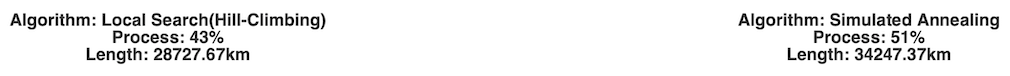
\includegraphics[width=\textwidth]{mid.png}
%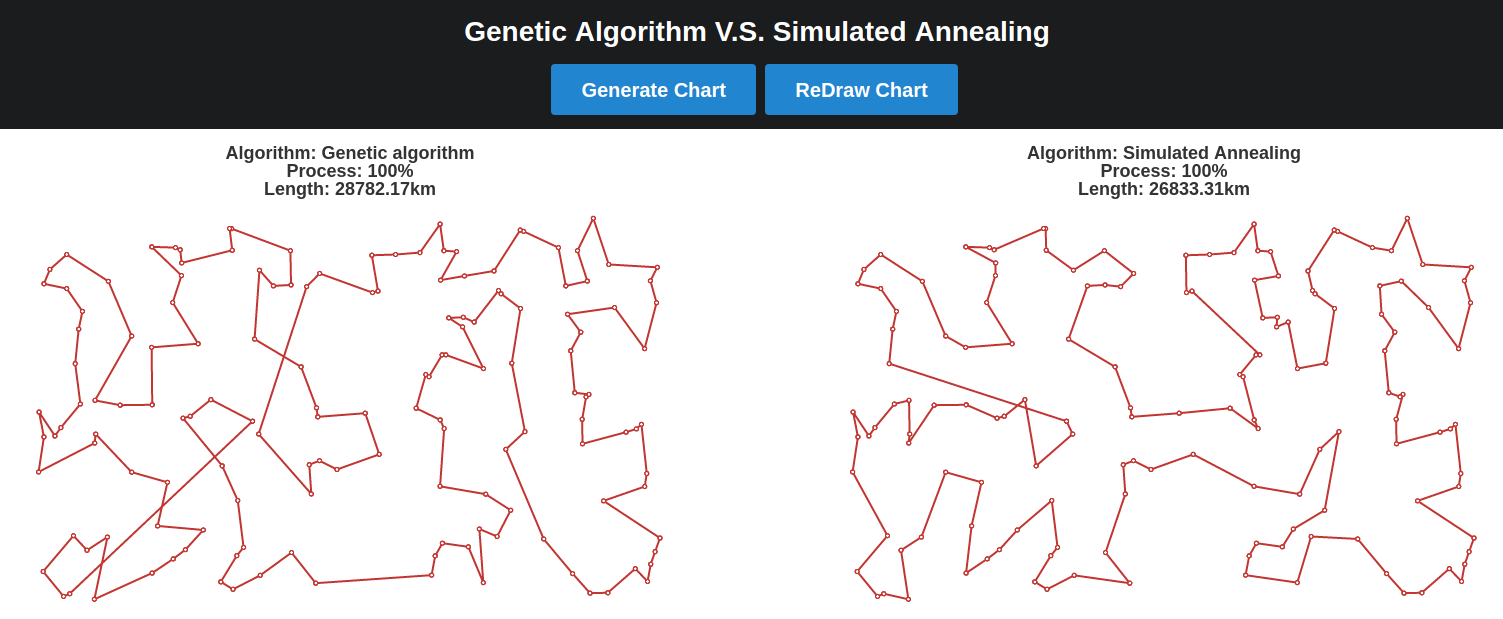
\includegraphics[width=\textwidth]{final.png}
%\caption{\label{fig:final}50\% 和 100\% 进度时结果.}
%\end{figure}

\subsubsection{模拟退火}


\subsubsection{遗传算法}


\subsection{对比与总结}

模拟退火算法和遗传算法都能够跑进最优解 10\% 的范围内,但是在使用相同局部搜索策略以及相同迭代数的情况下,模拟退火算法的表现整体上优于遗传算法。二者最终得到的解与参数设置有很强的关系,调参的不适当都有可能导致算法陷入局部最优解。

模拟退火算法由于是一种单点搜索算法,每轮迭代的操作相对简单,因此相同条件下的收敛时间也较短,对于一定概率下对非最优解的接受使得它通常能有效避开局部最优解。

遗传算法作为一种多点搜索算法,相同条件下其每轮迭代时间都较长。遗传算法能够避开局部最优解的关键在于其交叉和变异操作带来的种群个体多样性,并且在选择操作中对于非最优解也有一定的接受度。由于足够随机化的操作算子和多点搜索极强的全局搜索能力,遗传算法通常能够避开局部最优解。

通常情况下,模拟退火算法在相同的条件下可以具有比遗传算法更好的表现。

\end{document}